\chapter{Prélude: Cosmologie newtonienne\index{cosmologie Newtonienne}}

Ce chapitre est à la fois optionnel et indispensable : optionnel, car le reste de l'ouvrage n'en dépend pas et les quelques points qui y sont abordés sont décrits bien plus en détail dans les chapitres suivants. Il n'en reste pas moins indispensable en ce qu'il permet d'introduire facilement et simplement beaucoup de concepts utilisés couramment en cosmologie.

Ce prélude porte sur un modèle \textit{Newtonien} de cosmologie\index{cosmologie Newtonienne}. Ce modèle possède une portée limitée, mais permet une introduction progressive à certains concepts et à certains modes de raisonnements propres à la cosmologie. On discutera de sa validité et des hypothèses sous-jacentes en fin de chapitre, après en avoir exploré tous les recoins.

\newthought{Considérons} un «gaz de galaxies» \index{galaxie} homogène et isotrope au sein duquel on trace un volume sphérique de rayon $R$ et d'origine $O$. Au sein de ce volume, chacune de ces galaxies est repérée grâce à un rayon vecteur $r(t)$, variable au cours du temps (voir Fig. \ref{f:newton}). Ce modèle repose sur l'hypothèse que toutes ces galaxies vont voir leur position évoluer \textit{radialement} par rapport à $O$ suivant une loi homothétique:
\begin{equation}
r(t)=a(t)r_0.
\end{equation}
$r(t)$ est le rayon à un instant donné tandis que $r_0$ est le rayon mesuré pour chacune de ces galaxies à un instant arbitraire $t_0$. La dépendance temporelle est encodée dans le facteur d'échelle \index{facteur d'échelle}\sidenote{appelé aussi \textit{facteur d'expansion}}, $a(t)$. Ce dernier est un facteur sans dimension et dont on voit que par définition:
\begin{equation}
a(t_0)=a_0=1.
\end{equation}
Cet instant $t_0$ peut être choisi arbitrairement, mais il est d'usage de dire qu'il correspond au \textit{moment présent} : pour $t<t_0$ on regarde le système dans le passé et $t>t_0$ il s'agit du futur. De même, toute quantité indicée avec $0$ est prise à sa valeur aujourd'hui et par exemple $r(t_0)=r_0$.

\begin{figure}[htbp]
	\centering
		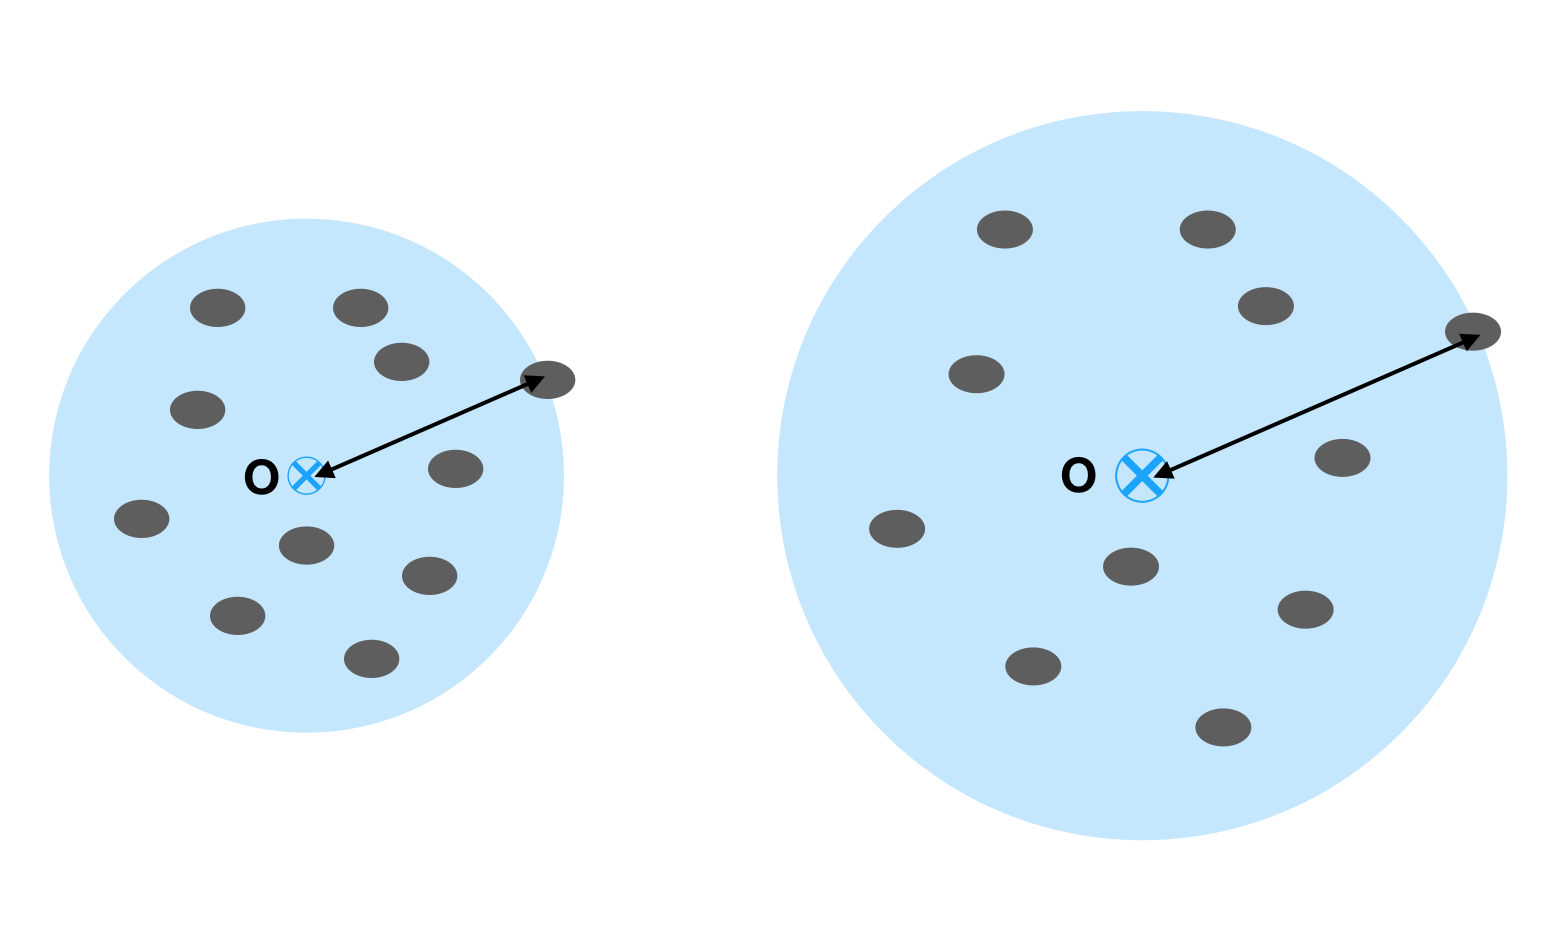
\includegraphics[height=6cm]{figs/newton.png}
	\caption[le modèle cosmologique Newtonien]{Le modèle Newtonien. La sphère représente une portion de gaz de galaxies, uniforme et isotrope centrée sur $O$. Seules quelques galaxies sont représentées ici sous forme d'ellipses : la plus éloignée d'entre elles fournit le rayon maximum de notre \textit{volume de contrôle} (montré ici sous la forme d'une flèche). Deux instants sont représentés ici, le temps s'écoulant de la gauche vers la droite et le volume subit alors une transformation homothétique. Notons que la galaxie la plus éloignée reste toujours la même à tous les instants.}
	\label{f:newton}
\end{figure}

Dès à présent, on peut constater que la notion de distance à l'origine n'est pas univoque : elle peut désigner la distance à un moment donné ou bien la distance variant au cours du temps. Pour lever cette ambiguïté, on appelle $r(t)$ \textit{la distance physique}\index{distance!physique}: à chaque instant elle représente l'intervalle qui sépare physiquement une galaxie de l'origine. De même on appelle $r_0$ la distance \index{distance!comobile} comobile : c'est la distance mesurée à un instant de référence $t_0$, mais on peut également la considérer comme une mesure effectuée dans un système de coordonnées en mouvement avec la matière (d'où le nom comobile). Enfin, le facteur d'expansion peut également être envisagé comme une mesure du rayon en unité du rayon comobile.

Si on considère maintenant le bord externe de notre volume de contrôle $R(t)$, celui-ci subit la même loi d'expansion\index{expansion} $R(t)=a(t)R_0$ \sidenote{se faisant on considère que ce rayon est «attaché» ou ancré à une galaxie, la galaxie la plus externe }. Ce volume de contrôle est sphérique, il évolue au cours du temps et son expression précise est:
\begin{equation}
V(t)=\frac{4\pi}{3} R(t)^3 = a(t)^3\frac{4\pi}{3} R_0^3= a^3 V_0.
\end{equation}
Son volume varie en $a^3$, comme tous les volumes attachés à de la matière. De même on peut aisément démontrer que sa surface varie en $a^2$ comme toutes les surfaces attachées à de la matière: dans les deux cas, la dépendance de ces quantités par rapport aux longueurs impose une certaine dépendance par rapport au facteur d'expansion. Ce type d'arithmétique est très fréquente en cosmologie et peut être aisément étendue à d'autres quantités, par exemple la densité de galaxies dans notre volume de contrôle:
\begin{equation}
n=\frac{N_\mathrm{gal}}{\frac{4\pi}{3} R(t)^3}=a^{-3} n_0.
\end{equation}
À cause de la dilution des longueurs et des volumes, la densité décroît au cours du temps avec une puissance $-3$ du facteur d'expansion. 

Notons dès à présent que la masse ou le nombre de galaxies restent invariants malgré l'évolution des distances. Dit autrement, le flux\index{flux} net au travers de la surface de contrôle est nul : aucune galaxie ne rattrape ou ne se fait dépasser par une galaxie initialement plus interne ou plus externe. En effet si $R_{0,a}<R_{0,b}<R_{0,c}$ alors à chaque instant $R_a<R_b<R_c$.

\newthought{La cinématique} de ce système mérite aussi d'être étudiée. La vitesse de fuite de chacune de ces galaxies est simplement donnée par:
\begin{equation}
\dot r= r_0 \dot a = \frac{\dot a}{a} r.
\end{equation}
À un instant $t$ donné, la vitesse de fuite\index{vitesse!fuite} est donc directement proportionnelle à la distance d'une galaxie : plus elle est éloignée de l'origine, plus elle s'en éloigne rapidement. Cela est cohérent avec l'absence de flux net au travers des limites du volume de contrôle. Le rapport de proportionnalité varie au cours du temps et est noté $H(t)$:
\begin{equation}
H(t)=\frac{\dot a}{a}.
\end{equation}
Dans ce cadre Newtonien, cette fonction est l'analogue à la fonction de Hubble \index{Hubble!fonction} que nous rencontrerons par la suite et nous retrouvons cette propriété observée dans notre univers. La vitesse de récession\index{vitesse!récession} des objets est proportionnelle à leur distance:
\begin{equation}
v=Hr
\label{e:hubblenewt}
\end{equation}
Cette loi dite \textit{de Hubble} est linéaire\index{linéaire}, ce qui a une grande importance. En effet, si la loi avait été quadratique ($v\sim r^2$) ou bien à vitesse de récession constante ($v\sim r^0$), on peut aisément montrer que l'homogénéité\index{homogénéité} initiale est détruite, ce qui n'est pas une propriété désirable de notre modèle d'Univers. Par ailleurs, on peut également démontrer que cette hétérogénéité serait dépendante du point de vue ou de l'origine utilisée, ce qui est une autre propriété indésirable. Cette loi de Hubble\index{Hubble!loi}, linéaire, est la seule qui permette de conserver une homogénéité et une égalité des points de vue.

\newthought{L'énergétique} du système nous est à présent accessible. Calculons la quantité d'énergie disponible dans ce gaz de galaxies, que ce soit sous forme cinétique ou potentielle. L' énergie cinétique \index{energie@énergie!cinétique} est obtenue en sommant l'énergie cinétique de chaque coquille de rayon $r$ et d'épaisseur $dr$ en récession \sidenote{$\rho$ désigne la densité massique de galaxies. Elle est indépendante de $r$, le système étant homogène}:
\begin{equation}
E_c=\int_0^R dE_c=\int_0^R \frac{1}{2}\rho  v^2(r) 4\pi r^2  dr.
\end{equation}
En utilisant la loi de Hubble (Eq. \ref{e:hubblenewt}) et la relation entre masse et densité, on obtient aisément l'expression suivante pour l'énergie cinétique totale du gaz en expansion\sidenote{M désigne la masse dans le volume de contrôle (conservée au cours du temps) et R le rayon de ce dernier}:
\begin{equation}
E_c=\frac{3}{10} M H^2 R^2.
\end{equation}
On y retrouve aisément une dépendance en vitesse au carré \sidenote{via le terme $Hr$}. De même l' énergie potentielle \index{energie@énergie!potentielle} totale de gravitation se trouve en intégrant l'énergie potentielle de chaque coquille \sidenote{l'énergie potentielle de gravitation est considérée nulle à l'infini. L'énergie potentielle d'une coquille de rayon $r$ ne dépend que de $M(<r)$, la masse à l'intérieur de son rayon. }:
\begin{equation}
E_p=\int_0^3 dE_p=-\int_0^R \frac{GM(<r)}{r}dm.
\end{equation}
Ayant $M(<r)=4/3\pi \rho r^3$ et $dm= 4\pi r^2 \rho dr$, on obtient:
\begin{equation}
E_p=-\frac{16 \pi^2 G}{3} \rho^2 \frac{R^5}{5}= -\frac{3}{5}\frac{GM^2}{R},
\end{equation} 
expression pour laquelle on retrouve bien une forme d'énergie potentielle de gravitation.

\section{Quelques éléments de dynamique}
Après avoir étudié ces quelques propriétés simples de notre modèle Newtonien, nous allons procéder à une première analyse de son évolution. Pour ce faire nous nous en tiendrons à une simple analyse énergétique. À partir des expressions des énergies cinétiques et potentielles, calculons l'énergie mécanique \index{energie@énergie!mécanique} totale de notre système auto-gravitant:
\begin{equation}
E=E_c+E_p=\frac{3}{10} M H^2 R^2 - \frac{3}{5}\frac{GM^2}{R}.
\end{equation}
Comme tout système auto-gravitant\index{système auto-gravitant}, sa stabilité nous est donnée par le signe de son énergie mécanique. Une énergie totale positive va conduire à un système libre, avec une expansion infinie (voire asymptotiquement infinie si elle est exactement nulle) tandis qu'une énergie négative correspond à celle d'un système lié, voué à s'effondrer au bout d'un certain temps.

\newthought{Quelle condition} faut-il satisfaire pour avoir un système lié ? Écrivons l'inégalité correspondante:
\begin{equation}
\frac{3}{10} M H^2 R^2 <\frac{3}{5}\frac{GM^2}{R}.
\end{equation}
Cette inégalité peut se réécrire sous la forme d'une condition sur la densité:
\begin{equation}
\frac{3H^2}{8\pi G}< \frac{M}{4/3\pi R^3}=\rho.
\end{equation}
Dit autrement si la densité de notre gaz de galaxies est supérieure à une certaine densité critique, le système est voué à atteindre un rayon limite et à s'effondrer. Cette densité critique \index{densité critique} est donnée par:
\begin{equation}
\rho_c =\frac{3H^2}{8\pi G}
\end{equation}
et correspond exactement à la densité critique obtenue par un traitement relativiste exact. De même on montrera qu'un gaz de galaxies sous- dense, avec $\rho< \rho_c$, n'est pas lié et  connaîtra une expansion illimitée. 

Compte tenu du rôle joué par cette densité critique, il est d'usage d'exprimer les densités massiques en unités de cette densité de référence. On parle alors de paramètre de densité \index{paramètre de densité} $\Omega$:
\begin{equation}
\Omega=\frac{\rho}{\rho_c}.
\end{equation}
Un système lié voué à l'effondrement équivaut à $\Omega>1$ tandis qu'un système en expansion infinie équivaut à $\Omega<1$. Le cas limite $\Omega=1$ correspond à un comportement asymptotique avec une expansion nulle à l'infini. À nouveau, cette relation sera très exactement retrouvée dans le cadre d'un traitement relativiste complet.

\section{Équation de Friedmann}

Ce paramètre de densité $\Omega$ intervient également dans l'équation différentielle qui régit l'évolution du facteur d'expansion $a(t)$\index{facteur d'échelle}. On rappelle que ce terme encode toute l'évolution temporelle des distances dans notre modèle Newtonien d'Univers, via la relation $r(t)=a(t)r_0$. Prenons la galaxie la plus lointaine\sidenote{ce choix est arbitraire, le même raisonnement peut être tenu pour n'importe quelle galaxie à l'intérieur du volume de contrôle}, dont la distance a l'origine est donnée par $R(t)$. Comme la mécanique newtonienne peut s'appliquer, le principe fondamental de la dynamique\index{principe fondamental de la dynamique} donne \sidenote{notons que le mouvement est purement radial en l'absence de mouvements initiaux tangentiels. $M(<R)$ désigne la masse à l'intérieur du rayon R et la force ressentie par la galaxie est celle crée par toute cette masse rassemblée en O.}:
\begin{equation}
\ddot R=-\frac{GM(<R)}{R^2}.
\end{equation} 
En l'absence de flux net au travers de $R$, la masse $M(<R)$ reste constante ce qui permet d'intégrer simplement en multipliant par $2\dot R$:
\begin{eqnarray}
2\dot R \ddot R &=& -2GM\frac{\dot R}{R^2}\\
\left(\frac{\dot R}{R}\right)^2&=&\frac{8\pi G}{3}\rho +\frac{K}{R^2}
\end{eqnarray}
où $K$ désigne une constante d'intégration. On reconnaît alors dans le terme de gauche le paramètre de Hubble $H=\dot a/a=\dot R/R$. Introduisons également la valeur de ce paramètre aujourd'hui $H_0=H(t_0)$ :
\begin{equation}
H^2=H_0^2(\frac{8\pi G}{3H_0^2}\frac{\rho_0}{a^3}+\frac{K}{(R_0  H_0)^2 a^2}).
\end{equation}
On reconnaît l'expression de la densité critique\index{densité critique} prise aujourd'hui $\rho_{c0}$ dans le terme lié à la densité de matière $\rho_0$. De plus le second terme lié à la constante d'intégration doit également être sans dimension et constant, à la dépendance en $a^{-2}$ près. Pour ces raisons, cette équation est généralement présentée sous la forme suivante:
\begin{equation}
H^2=H_0^2(\frac{\Omega_m}{a^3}+\frac{\Omega_K}{a^2}).
\label{e:friednewt}
\end{equation}
qui donne l'évolution du paramètre de Hubble\index{Hubble!fonction} au cours du temps \sidenote{via la dépendance temporelle en $a(t)$}, en fonction du contenu en masse, $\Omega_m$, de notre modèle d'Univers. La constante $K$ a généré un terme supplémentaire qui ne dépend que des conditions aux limites et qui doit satisfaire\sidenote{avec $H(a_0=1)=H_0$} :
\begin{equation}
\Omega_m+\Omega_K=1.
\end{equation}
Ce terme n'est pas libre et correspond à une quantité qui possède une dépendance en inverse de la longueur au carré\sidenote{par analogie avec le terme en densité qui varie en $a^{-3}$ alors que celui-ci varie en $a^{-2}$} : il correspond à un terme de courbure intrinsèque\index{courbure}. L'équation \ref{e:friednewt} contient toute l'information pour permettre de calculer $a(t)$, connaissant $\Omega_m$ et $H_0$: elle constitue l'une des formes de l'équation de Friedmann \index{equation@équation de Friedmann}.

\newthought{Prenons un Univers critique}: dans ce type de modèle, $\Omega_m=1$ et produit une dynamique que l'on sait être asymptotiquement en expansion pour un temps infini. L'équation \ref{e:friednewt} est alors très simple à intégrer à partir de \sidenote{ici on ne considère que la solution croissante, correspondant à l'Univers observé qui s'avère être en expansion}:
\begin{equation}
\dot a=\frac{H_0}{\sqrt{a}}
\end{equation}
ou bien
\begin{equation}
\sqrt{a}da=H_0 dt.
\end{equation}
En intégrant entre $t=0$ et un temps $t$ quelconque on obtient la loi d'expansion de ce modèle d'Univers:
\begin{equation}
a(t)=\left(\frac{3}{2}H_0 t\right)^{2/3}.
\end{equation}
On reconnaît une évolution temporelle lente asymptotique avec comme dérivées du facteur d'expansion:
\begin{eqnarray}
\dot a &\sim& t^{-1/3}\\
\ddot a &<&0.
\end{eqnarray}
La dérivée tend vers 0 à l'infini et la courbure est négative, donnant une expansion qui décélère : ce comportement est typique des Univers remplis de matière. Ce modèle est appelé modèle de \textit{Einstein-de Sitter} \index{Einstein- de Sitter}.

\newthought{L'âge de l'Univers}\index{age de l'Univers@âge de l'Univers} s'obtient également très facilement : il suffit de prendre le temps correspondant à un facteur d'échelle unité, c'est à dire le temps qu'il s'est écoulé depuis $t=0$:
\begin{equation}
t_0=\frac{2}{3H_0}.
\end{equation}
On constate alors que l'inverse du facteur de Hubble actuel est l'âge de l'Univers à un facteur proche de 1 près. De fait on nomme cette quantité le \textit{temps de Hubble}\index{Hubble!temps}\sidenote{Notons que la loi de Hubble $v=Hr$ suggérait déjà que $H$ constituait l'inverse d'un temps}:
\begin{equation}
t_H=H_0^{-1}.
\end{equation} 
Dans tous les modèles d'Univers, cette quantité constitue une bonne approximation de l'âge de l'Univers. De fait toute quantité temporelle qui est désignée comme étant de l'ordre du temps de Hubble \index{Hubble!temps} est implicitement désignée comme une quantité longue ou lente en évolution. C'est l'ordre de grandeur du temps caractéristique d'évolution de l'Univers.

Remarquons d'emblée que l'âge de l'Univers prédit par ce modèle simple est problématique. Pour une valeur typique de $H_0\sim 70$ km/s/Mpc \sidenote{correspondant à un temps de Hubble $t_H\sim 14$ milliards d'années}, le modèle d'Einstein-de Sitter conduit à un âge actuel d'Univers d'environ 9.2 milliards d'années or il existe des populations d'étoiles\sidenote{par exemple au sein d'amas globulaires\index{amas globulaire}} qui présentent des âges de plus de 13 milliards d'années. Ne pouvant avoir un Univers plus jeune que son contenu, il faut envisager autre chose qu'un Univers composé uniquement de matière avec une densité critique.

\section{Commentaire sur la validité du modèle}
À ce stade, on peut s'interroger sur les conditions d'applications de ce modèle Newtonien. Rappelons que nous considérons une sphère de «gaz» de galaxies dans un Univers homogène : il s'avère que dans certains cas, le traitement Newtonien est exact. En effet, faisons l'expérience de pensée qui consiste à retirer une sphère de matériau à cet ensemble homogène : quelle est la structure de l'espace-temps au sein de ce creux nouvellement créé ? La solution est donnée par le théorème de Birkhoff\index{théorème de Birkhoff} : l'espace-temps y est plat \sidenote{De la même façon, quel est le champ Newtonien de gravitation crée à l'intérieur d'une sphère creuse? D'après le théorème de Birkhoff, la réponse est un champ de gravitation nul, dont l'équivalent relativiste est une absence de courbure de l'espace-temps.}. Par conséquent lorsque la matière est remise dans ce creux la mécanique y est celle d'un espace plat\index{espace-temps!plat}, à savoir newtonienne.

Ceci n'est toutefois vrai qu'à certaines conditions, la première étant que la matière que nous remettons dans ce volume n'y courbe pas significativement l'espace afin que l'on puisse continuer à raisonner sans relativité générale. On peut par exemple imposer que l'énergie potentielle\index{energie@énergie!potentielle} de gravitation soit faible par rapport à son énergie de masse:
\begin{equation}
\frac{GM}{Rc^2}\ll 1
\end{equation}
Par ailleurs, il faut la taille de notre volume soit petite par rapport à l'horizon\index{horizon}, pour que les effets de propagation de l'interaction gravitationnelle \sidenote{qui se fait à la vitesse de la lumière} ne se fassent pas sentir:
\begin{equation}
\frac{RH}{c}\ll 1,
\end{equation}
ce qui est équivalent à considérer une vitesse de fuite très inférieure à la vitesse de la lumière. Donc de fait, le système ne peut être ni trop grand (pour éviter les grandes vitesses) ni trop petit (pour éviter les trop grandes densités). Par contre dans le cadre de ces hypothèses, le traitement est exact.

Une autre difficulté rencontrée par ce problème est qu'il est limité à l'action de la matière seule : qu'en est-il d'un modèle à l'intérieur duquel se trouve également du rayonnement ou bien toute autre forme d'énergie ? Le cadre Newtonien ne peut répondre à cette question or l'on comprend bien que ces autres types d'énergie doivent aussi contribuer à créer de la gravitation, comme indiqué par la relativité générale\index{relativité générale}. On peut faire appel de façon ad hoc à un résultat relativiste en disant que toute forme d'énergie va contribuer sous la forme d'une densité \textit{équivalente} de matière de la forme \sidenote{$\epsilon$ désigne la densité d'énergie associée à l'énergie en question et $P$ est sa pression}:
\begin{equation}
\tilde \rho= \frac{1}{c^2}(\epsilon + 3P).
\end{equation}
Dans le cas d'une matière froide\sidenote{sans pression}, on retrouve $\tilde \rho =\rho$. Pour le cas d'un gaz de rayonnement on peut démontrer que le la densité équivalente est $\tilde \rho =2\epsilon/c^2$. Par exemple pour un corps noir\index{corps noir} \sidenote{qui est l'exemple typique d'un gaz de photons fortement couplé avec la matière}, la densité d'énergie $\epsilon$ et la pression $P$\index{corps noir!pression} sont des fonctions simples de la température \index{corps noir!température} $T$\sidenote{ici $\sigma\sim 5.6\times10^{-8}Wm^{-2} K^{-4}$ désigne la constante de Stefan-Boltzmann}:
\begin{eqnarray}
\epsilon&=&\frac{4\sigma}{c} T^4\\
P&=&\frac{4\sigma}{3c} T^4.
\end{eqnarray}
Ces relations conduisent bien à la densité équivalente décrite ci-dessus. Toutefois, cette «astuce» ne permet pas d'expliquer quel rôle joue la pression et pourquoi elle contribue à modifier la dynamique de l'espace-temps. Cet aspect sera décrit plus en détail dans le chapitre suivant.

